\documentclass[a4paper, openany, 12pt]{article}

%% подключаем стандарт библиографии
\bibliographystyle{gost71u}

%% для "Abstract" в классе book
% \newenvironment{abstract}{}{}
% \usepackage{abstract}

%% подключаем преамбулу: в ней содержится подключение всех необходимых пакетов
%% Работа с русским языком
\usepackage{cmap}			 % поиск в PDF
\usepackage{mathtext} 		 % русские буквы в формулах
\usepackage[T1,T2A]{fontenc}
\usepackage[utf8]{inputenc}	 % кодировка исходного текста
\usepackage[russian]{babel}	 % локализация и переносы

%% Пакеты для работы с математикой
\usepackage{amsmath,amsfonts,amssymb,amsthm,mathtools}
\usepackage{icomma}

%% Нумерация формул (опционально)
%\mathtoolsset{showonlyrefs=true} % показывать номера только у тех формул, на которые есть \eqref{} в тексте.
%\usepackage{leqno}               % нумерация формул слева

%% Шрифты
\usepackage{euscript}	 % шрифт "Евклид"
\usepackage{mathrsfs}    % красивый мат. шрифт
\usepackage{setspace}
%% Некоторые полезные макросы для дебага (в случае недоверия авторам шаблона)
\makeatletter
\newcommand\thefontsize{The current font size is: \f@size pt} % пример: \section{\thefontsize}
\makeatother

%% Настройка размеров шрифтов
\makeatletter
\setlength{\headheight}{28pt}
%% TODO: мне не удалось разобраться, как грамотно подбирать второе число в
%% \@setfontsize\*, но ряд эксппериментов показывает, что "10" выравнивает текст весьма прилично :)
\renewcommand\Huge{\@setfontsize\Huge{14pt}{10}}
\renewcommand\huge{\@setfontsize\huge{14pt}{10}}
\renewcommand\Large{\@setfontsize\Large{14pt}{10}}
\renewcommand\large{\@setfontsize\large{12pt}{10}}
\makeatother

%% Поля (геометрия страницы)
\usepackage[left=3cm,right=1.5cm,top=3cm,bottom=2cm,bindingoffset=0cm]{geometry}

%% Русские списки
\usepackage{enumitem}
\makeatletter
\AddEnumerateCounter{\asbuk}{\russian@alph}{щ}
\makeatother

%% Работа с картинками
\usepackage{caption}
\captionsetup{justification=centering} % центрирование подписей к картинкам
\usepackage{graphicx}                  % вставки рисунков
\graphicspath{{images/}{images2/}}     % папки с картинками
\setlength\fboxsep{3pt}                % отступ рамки \fbox{} от рисунка
\setlength\fboxrule{1pt}               % толщина линий рамки \fbox{}
\usepackage{wrapfig}                   % обтекание рисунков и таблиц текстом

%% Работа с таблицами
\usepackage{array,tabularx,tabulary,booktabs} % дополнительная работа с таблицами
\usepackage{longtable}                        % длинные таблицы
\usepackage{multirow}                         % слияние строк в таблице

%% Красная строка
\setlength{\parindent}{2em}

%% Интервалы
\linespread{1}
\usepackage{multirow}

%% TikZ
\usepackage{tikz}
\usetikzlibrary{graphs,graphs.standard}

%% Верхний колонтитул
\usepackage{fancyhdr}
\pagestyle{fancy}

%% Перенос знаков в формулах (по Львовскому)
\newcommand*{\hm}[1]{#1\nobreak\discretionary{}{\hbox{$\mathsurround=0pt #1$}}{}}

%% Дополнительно
\usepackage{float}   % добавляет возможность работы с командой [H] которая улучшает расположение на странице
\usepackage{gensymb} % красивые градусы
\usepackage{caption} % пакет для подписей к рисункам, в частности, для работы caption*
\usepackage{listings} % пакет для листингов с кодом

% Hyperref (для ссылок внутри  pdf)
\usepackage[unicode, pdftex]{hyperref}

% Отступ перед первым абзацем в каждом разделе
\usepackage{indentfirst}

\usepackage[russian]{babel}
\usepackage{geometry}
\geometry{left=3cm,right=1.5cm,top=2cm,bottom=2cm, headheight=2cm, headsep=0.5cm}

\usepackage{xcolor}

\usepackage{titlesec}

% Настройка размеров (можно использовать конкретные pt)
\titleformat{\section}
  {\normalfont\fontsize{17}{19}\bfseries}{\thesection}{1em}{}

\titleformat{\subsection}
  {\normalfont\fontsize{15}{17}\bfseries}{\thesubsection}{1em}{}

\titleformat{\subsubsection}
  {\normalfont\fontsize{14}{15}\bfseries}{\thesubsubsection}{1em}{}

% Интервалы вокруг заголовков
\titlespacing*{\section}{0pt}{12pt}{6pt}
\titlespacing*{\subsection}{0pt}{10pt}{4pt}
\titlespacing*{\subsubsection}{0pt}{10pt}{4pt}

\definecolor{codegreen}{rgb}{0,0.6,0}
\definecolor{codegray}{rgb}{0.5,0.5,0.5}
\definecolor{codepurple}{rgb}{0.58,0,0.82}


\lstdefinestyle{mystyle}{
    commentstyle=\color{codegreen},
    keywordstyle=\color{magenta},
    numberstyle=\tiny\color{codegray},
    stringstyle=\color{codepurple},
    basicstyle=\ttfamily\footnotesize,
    breakatwhitespace=false,
    breaklines=true,
    captionpos=b,
    keepspaces=true,
    numbers=left,
    numbersep=5pt,
    showspaces=false,
    showstringspaces=false,
    showtabs=false,
    tabsize=2,
    frame=lines,
    inputencoding=utf8,
    extendedchars=\true,
    }


\lstset{style=mystyle}
\newcommand{\code}[1]{\texttt{#1}}

\usetikzlibrary{shapes,arrows,positioning}
\usepackage{lipsum} % Для демонстрации текста


% Определение стиля для TypeScript
\lstdefinelanguage{TypeScript}{
    keywords={let, const, type, interface, class, function, return, if, else, for, while, import, export},
    sensitive=true,
    comment=[l]{//},
    morecomment=[s]{/*}{*/},
    morestring=[b]',
    morestring=[b]",
    alsoletter={-},
    morekeywords=[2]{number, string, boolean, any, void, null, undefined}
}

\lstset{
    basicstyle=\ttfamily\small,
    keywordstyle=\color{blue},
    commentstyle=\color{green!50!black},
    stringstyle=\color{red},
    numbers=left,
    numberstyle=\tiny\color{gray},
    stepnumber=1,
    numbersep=5pt,
    backgroundcolor=\color{white},
    showspaces=false,
    showstringspaces=false,
    showtabs=false,
    tabsize=2,
    captionpos=b,
    breaklines=true,
    breakatwhitespace=true,
    frame=single,
    inputencoding=utf8,
    extendedchars=\true
    }

\usepackage{csquotes}
\usepackage[style=gost-numeric,  % Стиль по ГОСТ (или другой)
            backend=biber,      % Используем Biber вместо BibTeX
            sorting=none,       % Порядок цитирования
            language=auto]{biblatex}
\addbibresource{references.bib}



\begin{document}
    %% титульник
    \begin{center}
    %% *название института*
    \large\textbf{Министерство образования и науки Российской Федерации \\
    Московский физико-технический институт (государственный
    университет)} \\
    \vspace{1cm}

    %% *факультет/физтех-школа*
    Физтех-школа радиотехники и компьютерных технологий \\

    %% *название базовой кафедры и лаборатории*
    %% в случае ненадобности можно удалить
    Кафедра микропроцессорных технологий в интеллектуальных системах управления \\

    \vspace{3em}

    Выпускная квалификационная работа бакалавра
\end{center}

\begin{center}
    \vspace{\fill}
    %% *название вашей работы*
    \LARGE{Удаление примитивных типов из высокоуровневого языка программирования для улучшения качества семантического анализа}

    \vspace{\fill}
\end{center}


\begin{flushright}
    \textbf{Автор:} \\
    Студентка группы Б01-109а \\
    Ермолаева Варвара Дмитриевна \\
    \vspace{2em}
    \textbf{Научный руководитель:} \\
    Солдатов Антон Анатольевич \\
    \vspace{2em}
    \textbf{Научный консультант:} \\
    Солдатов Антон Анатольевич \\
\end{flushright}

\vspace{7em}

\begin{center}
    %% *лого*
    \includegraphics[width=100 pt]{MIPT_logo.jpg}\\
    Москва \the\year{}
\end{center}

%% выключаем отображение номера для этой страницы (титульник)
\thispagestyle{empty}

\newpage
\setcounter{page}{2}
\fancyfoot[c]{\thepage}
%% *надпись над верхним колонтинулом*
%% в случае ненадобности можно удалить
\fancyhead[L]{Удаление примитивных типов из высокоуровневого языка программирования для улучшения качества семантического анализа}
\fancyhead[R]{}
    %% аннотоция
    
\begin{center}
\subsubsection*{Удаление примитивных типов из высокоуровневого языка программирования для улучшения качества семантического анализа}
\textbf{Ермолаева Варвара Дмитриевна}
\end{center}

В современных управляемых языках программирования (таких как Java, C\#, Kotlin) сохраняется исторически сложившееся разделение типов на примитивные (например, \texttt{int}, \texttt{boolean}) и объектные (ссылочные). Это разделение, хотя и направлено на повышение производительности, приводит к:

\begin{itemize}[leftmargin=*,label={--}]
    \item Несогласованности в системе типов
    \item Усложнению семантического анализа
    \item Ограничению возможностей объектно-ориентированного программирования (например, отсутствие полиморфизма для примитивов, необходимость упаковки/распаковки)
\end{itemize}

\medskip

Целью данной работы является улучшение качества семантического анализа за счёт устранения дуализма примитивных и объектных типов в высокоуровневом языке программирования с управляемой средой исполнения. Для этого предложена стратегия <<Примитивы как оптимизация компилятора>>, при которой:

\begin{itemize}[leftmargin=*,label={--}]
    \item Все типы унифицируются в рамках объектной модели
    \item Примитивные операции выполняются непосредственно над объектами (например, \texttt{Int} вместо \texttt{int})
    \item Низкоуровневые оптимизации (замена объектов на примитивы) выполняются на этапе компиляции, не влияя на семантику языка
\end{itemize}

\medskip

В работе проведён:

\begin{itemize}[leftmargin=*,label={--}]
    \item Анализ существующих подходов (Java, C\#, Kotlin)
    \item Разработана формальная спецификация унифицированной системы типов
    \item Реализованы:
    \begin{itemize}
        \item Модификации семантического анализа для поддержки объектных примитивоподобных типов
        \item Алгоритмы свёртки констант и преобразования типов
        \item Механизм оптимизации AST для замены объектов на примитивы
    \end{itemize}
\end{itemize}

\medskip

Результаты показали, что предложенное решение:

\begin{itemize}[leftmargin=*,label={--}]
    \item Упрощает семантический анализ за счёт устранения специальных правил для примитивов
    \item Сохраняет производительность благодаря оптимизациям на этапе компиляции
    \item Повышает удобство разработки, обеспечивая единообразие типов
\end{itemize}

\textbf{Ключевые слова:} система типов, примитивные типы, семантический анализ, оптимизация компилятора, унификация типов.

\newpage
    %% содержание
    \tableofcontents{}
    \newpage

    % \fontsize{14}{16}\selectfont
    \section{Введение}
\label{sec:Chapter0} \index{Chapter0}
\onehalfspacing % Полуторный интервал

Типовая система языка программирования служит фундаментом для формального определения его спецификации, обеспечивает статический анализ программ,
поддержку оптимизаций кода и способствует улучшению его структурированности и читаемости.
Высокоуровневые языки программирования(Java, C\#, Kotlin) предоставляют разработчику мощные абстракции и безопасность кода посредством автоматического
управления памятью и объектно-ориентированных парадигм. Многие из этих языков сохранили в себе исторически сложившееся разделение типов на "примитивные" типы и ``объектные''
или ``ссылочные'', призванное потенциально улучшить производительность в некоторых случаях. Тем не менее, в то же время оно приводит к несогласованности в системе типов и
усложняет достижение полностью единообразной и интуитивной модели программирования. Примитивные типы часто лишены полезных свойств объектов, таких как наследование,
полиморфизм, вызов методов без явного упаковывания/распаковывания и использование в качестве аргумента для шаблонных типов.

В данной работе будут теоретически рассмотрены последствия устранения явной разницы между примитивными и объектными типами из высокоуровневого управляемого языка
программирования и описаны этапы и результаты реализации.

\subsection{Типовая система}

Типовая система — это формальная синтаксическая и семантическая структура, сопоставляющая типы и программные конструкции (выражения, переменные, функции) для обеспечения чётко определённого вычислительного поведения. Её основные теоретические и практические назначения:

\begin{enumerate}[label=\arabic*), leftmargin=*]
    \item \textbf{Корректность поведения программы}

    С введением типовой системы становится возможной статическая верификация соблюдения ограничений типов, не допускающая к выполнению неверно типизированные программы. Данный механизм гарантирует:

    \begin{itemize}
        \item \textit{Безопасность выполнения} — предотвращение неопределённого поведения за счёт блокировки запрещённых операций (например, некорректные обращения к памяти в управляемых средах типа JVM/CLR)
        \item \textit{Теоретическую обоснованность} — соответствие двум фундаментальным принципам типобезопасности по Райту-Феллейзену:
        \begin{enumerate}[label=\arabic*., leftmargin=*]
            \item \textbf{Прогресс}: корректно типизированная программа не может застрять в промежуточном состоянии
            \item \textbf{Сохранение}: типы остаются согласованными на всех этапах вычисления
        \end{enumerate}
    \end{itemize}

    \item \textbf{Уровень абстракции кода}

    Типовая система обеспечивает инкапсуляцию доменных инвариантов с помощью абстракций типов (абстрактные типы данных и интерфейсы) и позволяет формально специфицировать границы модулей.

    \item \textbf{Возможность оптимизаций}

    Наличие статической типизации позволяет применять оптимизации на этапе компиляции (например, специализация обобщённых типов и статическое разрешение методов) и минимизировать время исполнения в управляемых средах за счёт уменьшения количества динамических проверок типов.
\end{enumerate}

\subsection{Статическая и динамическая типизации}

\begin{enumerate}[label=\arabic*., leftmargin=*]
    \item \textbf{Статическая типизация} (Java, C\#, Kotlin):
    \begin{itemize}
        \item Валидность типа доказывается на этапе компиляции с помощью формальных суждений о принадлежности выражения к типу в данном контексте ($\Gamma \vdash e : \tau$)
        \item Гарантирует типобезопасность по Райту-Феллейзену
        \item Критично для управляемых языков программирования из-за возможности проверок безопасности памяти (например, верификатор байт-кода JVM) и эффективности Just-In-Time компиляции за счёт встраивания методов, ориентированных на конкретный тип
    \end{itemize}

    \item \textbf{Динамическая типизация} (Python, JavaScript):
    \begin{itemize}
        \item Типы функций и выражений определяются во время исполнения
        \item Нет формальной гарантии типобезопасности, но есть возможность менять поведение объектов, модулей и классов во время исполнения
    \end{itemize}
\end{enumerate}

Современные управляемые языки высокого уровня (Java, C\#) преимущественно основаны на статической типизации, расширенной возможностями динамического анализа во время выполнения. Данный компромиссный подход позволяет сочетать строгость формальной верификации с практической гибкостью разработки, но противоречие между статическими гарантиями и динамической адаптируемостью продолжает оставаться предметом активных исследований.

\newpage



\subsection{Примитивные типы}

\subsubsection{Определение}

\textbf{Примитивные типы} (далее -- примитивные типы или примитивы) являются наиболее фундаментальным типом данных в языках программирования. В отличие от объектов, они:

\begin{itemize}
    \item \textbf{Не ссылают на память}, а непосредственно являются значениями, обычно находящимися на стеке. У них отсутствуют:
    \begin{itemize}
        \item заголовок объекта (object header)
        \item таблица виртуальных методов (vtable)
        \item ссылочная идентичность (identity)
    \end{itemize}

    \item Имеют \textbf{фиксированную семантику}, определяющуюся стандартами языка (например, Java JLS §4.2, C\# ECMA-334 §8.3)

    \item \textbf{Не могут быть подтипами} или наследоваться и являются атомарными (базовыми) элементами в иерархии типов
\end{itemize}

\subsubsection{Теоретический контекст}
В теории типов примитивы являются простейшими случаями конструирования типа и не разлагаются на более простые типы. Конструирование сложных типов происходит на основе:

\begin{itemize}
    \item \textbf{Произведения} (кортежи, записи) -- (Int, Bool)
    \item \textbf{Суммы} (типы-суммы, перечисления) -- \texttt{data Maybe a = Nothing | Just a}
    \item \textbf{Функции} -- Int → Bool
    \item \textbf{Рекурсивные типы} -- \texttt{data List a = Nil | Cons a (List a)}
\end{itemize}

\subsubsection{Основные характеристики}

\begin{itemize}
    \item \textbf{Представление в памяти}
    \begin{itemize}
        {Аллокация на стеке}* (default for local variables in methods)
    \end{itemize}
    \item \textbf{Производительность на уровне процессора}
    \begin{enumerate}
        \item

        Арифметические операции с примитивами компилируются непосредственно в нативные инструкции:

        \begin{lstlisting}[language={[x86masm]Assembler}]
    ; x86 assembly for 'a + b'
    mov eax, [a]
    add eax, [b]
        \end{lstlisting}

        \item \textbf{Локализация в кэше}

        Линейная модель доступа к памяти (критично для больших вычислений)
    \end{enumerate}
\end{itemize}

\subsubsection{Примеры в высокоуровневых языках -- NEED TO BE FIXED}

\begin{table}[h]
    \centering
    \caption{Примитивные типы в различных языках программирования}
    \begin{tabular}{lccc}
        \toprule
        \textbf{Тип} & \textbf{Java} & \textbf{C\#}  \\
        \midrule
        Целые числа & \texttt{int}, \texttt{long} & \texttt{int}, \texttt{long} \\
        Числа с плавающей & \texttt{float}, \texttt{double} & \texttt{float}, \texttt{double}  \\
        Булевы значения & \texttt{boolean} & \texttt{bool} \\
        Символ & \texttt{char} & \texttt{char} \\
        \bottomrule
    \end{tabular}
\end{table}


\subsubsection{Роль примитивных типов в управляемых средах исполнения}

\begin{itemize}
    \item \textbf{Специальные байт-код инструкции}:
    \begin{itemize}
        \item В JVM: \texttt{iload}, \texttt{iadd}, \texttt{fstore} для операций с \texttt{int}, \texttt{float} и др.
        \item В CLR: аналогичные IL-команды (\texttt{ldc.i4}, \texttt{add})
    \end{itemize}

    \item \textbf{Оптимизации времени исполнения}:
    \begin{itemize}
        \item Escape-анализ: Размещение временных переменных на стеке вместо кучи
        \item Интринсики: Замена вызовов методов (например, \texttt{Math.sin()}) на нативные CPU-инструкции
    \end{itemize}
\end{itemize}
 %% Введение
    \newpage
\section{Постановка задачи}
\label{sec:Chapter1} \index{Chapter1}

\subsection{Контекст}
В данной работе речь пойдет о высокоуровневом языке программирования с управляемой средой исполнения, поддерживающей два языка программирования~--- статически типизированный язык, похожий в большей степени на TypeScript, и динамически типизированный, схожий с JavaScript.

Язык поддерживает императивные, объектно-ориентированные, функциональные и шаблонные паттерны программирования и комбинирует разные семантические аспекты TypeScript, Java и Kotlin. На данный момент язык находится в активной стадии разработки.

Примитивные типы в разрабатываемом языке обладают основными характеристиками, описанными ранее~--- они:
\begin{itemize}
    \item не участвуют в подтипировании (в том числе с типом \code{Object})
    \item не могут быть компонентами юнион-типов
    \item не могут приниматься в шаблонных в качестве аргумента
    \item не имеют методов и других свойств объектов
\end{itemize}

Для обеспечения указанной функциональности язык предоставляет объектные аналоги примитивных типов (далее - объектные аналоги примитивных типов, примитивоподобные объекты), представляющие собой объектную обертку с соответствующими методами и правилами наследования (например, \code{Int}~--- объектный аналог примитивного типа \code{int}).
В случаях необходимости между примитивным типом и его аналогом происходит скрытая конверсия, что усложняет семантический анализ программ. Более того, синтаксически допускаются конструкции вида \code{int | undefined} или \code{Set<int>}, которые интерпретируются компилятором как \code{Int | undefined} и \code{Set<Int>}. Несоответствие свойств \code{int} и \code{Int} приводит к непредвиденному поведению в краевых случаях.

Далее в тексте \code{int} и \code{Int} будут использоваться в качестве основного примера.

\vspace{0.5cm}
\noindent\textbf{Цель работы:} улучшение семантического анализа программ посредством устранения концепции примитивных типов как отдельной категории и унификации системы типов.

\subsection{Задачи исследования}
Для достижения поставленной цели необходимо решить следующие задачи:
\begin{enumerate}[leftmargin=*,align=left]
    \item[\textbf{1.}] Провести детальный анализ текущего состояния семантического анализа с целью идентификации мест, где наличие примитивных типов приводит к:
    \begin{itemize}[label={--}]
        \item усложнению логики анализа
        \item неоднозначности интерпретации
        \item необходимости специальных правил обработки (скрытые конверсии, union-типы, generics)
    \end{itemize}

    \item[\textbf{2.}] Разработать формальную спецификацию унифицированной системы типов, которая:
    \begin{itemize}[label={--}]
        \item исключает концепцию примитивных типов
        \item интегрирует их функциональность в объектную модель
        \item сохраняет производительность операций (арифметические, логические)
        \item обеспечивает корректность семантики
    \end{itemize}

    \item[\textbf{3.}] Спроектировать и реализовать модификации в подсистеме семантического анализа, обеспечивающие:
    \begin{itemize}[label={--}]
        \item проверку совместимости типов
        \item разрешение перегрузок
        \item вывод типов
        \item работу с метаданными
    \end{itemize}

    \item[\textbf{4.}] Разработать набор тестовых сценариев, охватывающих:
    \begin{itemize}[label={--}]
        \item шаблонные с числовыми аргументами
        \item union-типы
        \item операции с числовыми значениями
        \item проблемные краевые случаи
    \end{itemize}

    \item[\textbf{5.}] Оценить влияние решения на:
    \begin{itemize}[label={--}]
        \item сложность и точность семантического анализа
        \item удобство разработки
        \item потенциальную производительность
    \end{itemize}
    с использованием формальных метрик:
    \begin{itemize}[label={--}]
        \item уменьшение количества специальных правил
        \item сокращение ветвлений в коде анализатора
        \item результаты тестовых сценариев
    \end{itemize}
\end{enumerate}

\subsection{Требования к решению}
\subsubsection{Функциональные требования}
\begin{enumerate}[leftmargin=*,align=left]
    \item[\textbf{1.}] \textbf{Унификация системы типов:} Разработанное решение должно обеспечить:
    \begin{itemize}[label={--}]
        \item полную интеграцию всех типов (числовых, логических) в общую объектную иерархию
        \item участие базовых типов в механизмах подтипирования
        \item устранение разделения на примитивные и объектные типы
    \end{itemize}

    \item[\textbf{2.}] \textbf{Поддержка продвинутых конструкций:} Все типы должны корректно использоваться в:
    \begin{itemize}[label={--}]
        \item \textbf{Union-типах:} конструкции вида \code{number | undefined} или \code{boolean | null} должны быть валидными
        \item \textbf{Дженериках:} базовые типы как аргументы (\code{Set<number>}, \code{Map<string, boolean>}) без скрытых преобразований
        \item \textbf{Наследовании/Подтипировании:} соблюдение общих правил для базовых типов
    \end{itemize}

    \item[\textbf{3.}] \textbf{Устранение скрытых конверсий:} Необходимо исключить:
    \begin{itemize}[label={--}]
        \item автоматические механизмы упаковки (boxing)
        \item автоматическую распаковку (unboxing) значений
        \item неявные преобразования между разными представлениями типов
    \end{itemize}

    \item[\textbf{4.}] \textbf{Семантическая корректность:} Анализатор должен обеспечивать:
    \begin{itemize}[label={--}]
        \item точное выявление типовых ошибок
        \item однозначное разрешение типов в выражениях
        \item предсказуемое поведение программ
    \end{itemize}

    \item[\textbf{5.}] \textbf{Сохранение синтаксиса:} Требуется:
    \begin{itemize}[label={--}]
        \item сохранить существующий синтаксис (\code{int}, \code{number}, \code{boolean})
        \item обеспечить соответствие внутренней интерпретации унифицированной модели
    \end{itemize}
\end{enumerate}

\subsubsection{Нефункциональные требования}
\begin{enumerate}[leftmargin=*,align=left]
    \item[\textbf{1.}] \textbf{Производительность:}
    \begin{itemize}[label={--}]
        \item отсутствие существенного замедления семантического анализа
        \item оптимизация алгоритмов проверки типов
    \end{itemize}

    \item[\textbf{2.}] \textbf{Эффективность кода:}
    \begin{itemize}[label={--}]
        \item отсутствие заметного снижения производительности исполняемого кода
        \item сравнимая эффективность с оригинальной реализацией
    \end{itemize}

    \item[\textbf{3.}] \textbf{Качество кода анализатора:}
    \begin{itemize}[label={--}]
        \item повышение читаемости и поддерживаемости
        \item модульная структура
        \item упрощение логики обработки типов
    \end{itemize}

    \item[\textbf{4.}] \textbf{Удобство разработки:}
    \begin{itemize}[label={--}]
        \item интуитивно понятная модель типов
        \item снижение когнитивной нагрузки
        \item минимизация неочевидных ошибок
    \end{itemize}
\end{enumerate}

\subsection{Ожидаемые результаты}
В результате выполнения дипломной работы ожидается получить:

\begin{itemize}
    \item \textbf{Спецификацию унифицированной системы типов} для высокоуровневого управляемого языка, включающую:
    \begin{itemize}[label={--}]
        \item формальное описание типовой системы
        \item правила подтипирования
        \item алгоритмы проверки типов
    \end{itemize}

    \item \textbf{Модифицированную подсистему семантического анализа} с:
    \begin{itemize}[label={--}]
        \item поддержкой унифицированных типов
        \item устранением специальных случаев для примитивов
        \item улучшенной архитектурой
    \end{itemize}

    \item \textbf{Комплекс тестовых примеров}, покрывающих:
    \begin{itemize}[label={--}]
        \item базовые операции с типами
        \item union-типы и шаблонные типы
        \item краевые случаи
        \item производительность анализа
    \end{itemize}

    \item \textbf{Оценочные метрики} по:
    \begin{itemize}[label={--}]
        \item сложности семантического анализа
        \item эффективности работы компилятора
        \item удобству использования языка
    \end{itemize}
\end{itemize}

\newpage
 %% Постановка задачи
    \section{Обзор существующих решений}
\label{sec:Chapter2} \index{Chapter2}

\subsection*{Интеграция примитивных типов в высокоуровневую систему типов и их влияние на семантический анализ}

\subsection{Явное разделение с автоматическим преобразованием}

\begin{itemize}[label={--}]
    \item \textbf{Суть:} Примитивные типы (`int`, `float`, `boolean`) и объектные типы (`Integer`, `Float`, `Boolean`) существуют параллельно и явно различимы в системе типов языка. Компилятор автоматически вставляет преобразования (боксинг - примитив -> объектная обертка, анбоксинг - объектная обертка -> примитив) там, где контекст требует типа другого вида (например, передача `int` в метод, ожидающий `Object`, или использование `Integer` в арифметической операции). Например, о гибридном подходе в CLR можно узнать из \cite{richter2012}.

    \item \textbf{Влияние на систему типов:}
    \begin{itemize}
        \item Явный дуализм типов
        \item Примитивы не являются частью объектной иерархии
        \item Необходимость учёта примитивных типов в правилах подтипирования
    \end{itemize}

    \item \textbf{Влияние на семантический анализ:}
    \textbf{Значительно усложняет анализ}
    \begin{itemize}[label={--}]
        \item Отслеживание контекстов, требующих преобразований
        \item Разрешать перегрузки методов с примитивными и объектными параметрами (иногда приводя к неочевидному выбору)
        \item Обрабатывать потенциальные \code{NullPointerException} при анбоксинге \code{null}
        \item Учитывать различия в семантике (например,  \code{==} для примитивов vs. для объектов)
        \item Иметь отдельные ветви кода для проверки типов примитивов и объектов
    \end{itemize}

    \item \textbf{Преимущества:}
    Позволяет использовать примитивы для производительности и объектные обертки там, где нужна полиморфность (коллекции). Понятна разработчикам низкого уровня.

    \item \textbf{Недостатки:} Сложная система типов и семантический анализ, риск ошибок `NullPointerException` из-за неявного анбоксинга, потенциальные накладные расходы на преобразования, концептуальный разрыв для разработчика. Также накладные расходы на boxing/unboxing в Java могут достигать 20\% производительности (см. \cite{chen2019})

    \item \textbf{Примеры:} Java (классический пример), ранние версии C\#
\end{itemize}

\newpage

\begin{lstlisting}[language=java,title=Пример в Java]
Integer x = 10;  // Автобоксинг
int y = x;       // Автоанбоксинг
if (y == x) {    // Сравнение с автоанбоксингом
    System.out.println("Equal");
}
\end{lstlisting}

\subsection{Единая иерархия типов с значимыми типами}

\begin{itemize}[leftmargin=*, label={--}]
    \item \textbf{Суть:} Примитивные типы реализованы как \textbf{значимые типы (value types)}, которые являются частью единой объектной иерархии типов (например, наследуются от базового класса \texttt{ValueType}, который сам наследуется от \texttt{Object}). Все типы (и ссылочные, и значимые) формально являются подтипами Object. Однако, между ссылочными (классы) и значимыми (структуры, примитивы) типами сохраняется фундаментальное различие в семантике: передача по ссылке и передача по значению (копированию), размещение в куче и в стеке/встроенно.

    \item \textbf{Влияние на систему типов:} Формально единая иерархия, но с глубоким внутренним разделением. Примитивы/значимые типы могут реализовывать интерфейсы. Возможно ограниченное наследование для значимых типов (или его отсутствие).

    \item \textbf{Влияние на cемантический aнализ:}
    \textbf{Усложнен.}
    Анализатор должен:
    \begin{itemize}
        \item Различать ссылочные и значимые типы на протяжении всего анализа.
        \item Учитывать семантику копирования при присваивании и передаче в методы для значимых типов.
        \item Обрабатывать боксинг/анбоксинг (упаковку/распаковку) при необходимости преобразования значимого типа в ссылочный (\code{object}, интерфейс) и обратно, со всеми вытекающими последствиями (накладные расходы, \texttt{Null}?).
        \item Учитывать различия в поведении операторов (например, \code{==} по умолчанию для значимых типов сравнивает значения, а для ссылочных - ссылки).
    \end{itemize}

    \item \textbf{Преимущества:} Более единообразная модель типов, чем в Java. Значимые типы позволяют создавать эффективные пользовательские структуры данных. Возможность полиморфизма через интерфейсы.

    \item \textbf{Недостатки:} Сохраняется концептуальная сложность разделения ref/value. Семантический анализ все еще должен обрабатывать два разных вида типов и преобразования между ними. Риск неочевидных накладных расходов на упаковку.

    \item \textbf{Примеры:} C\# (структуры \code{struct}, примитивы как псевдонимы для системных структур типа \code{System.Int32}), Swift (value semantics для структур и перечислений).
\end{itemize}


\subsection{Примитивы как оптимизация компилятора}
\begin{itemize}[label={--}, leftmargin=*]
    \item \textbf{Суть:} Система типов языка оперирует только высокоуровневыми объектными типами. Примитивные типы абстрагированы на уровне семантики языка. Компилятор на поздних стадиях (после семантического анализа) агрессивно оптимизирует использование этих объектов:
    \begin{itemize}[label={--}]
        \item заменяет их на низкоуровневые примитивные значения,
        \item подставляет реализацию их методов напрямую в код,
        \item устраняет накладные расходы на вызовы методов и выделение памяти.
    \end{itemize}
    Примитив используется только как реализационная деталь оптимизации, невидимая для семантики языка.

    \item \textbf{Влияние на cистему типов:} \textbf{Единая объектная модель.} Примитивы представлены как специальные неизменяемые объектные типы (часто \code{final} классы или \code{inline} классы). Для системы типов и разработчика они:
    \begin{itemize}[label={--}]
        \item выглядят и ведут себя как обычные объекты,
        \item имеют методы,
        \item могут быть упакованы в общие интерфейсы.
    \end{itemize}

    \item \textbf{Влияние на семантический Анализ:} \textbf{Существенно упрощен.} Анализатор работает исключительно с объектными типами. Нет необходимости:
    \begin{itemize}[label={--}]
        \item Различать примитивы и объекты при проверке типов.
        \item Обрабатывать правила боксинга/анбоксинга (их нет на уровне семантики).
        \item Беспокоиться о \code{NullPointerException} для самих объектных аналогов примитивов.
    \end{itemize}

    \item \textbf{Преимущества:}
    \begin{itemize}[label={--}]
        \item Максимально простая и единообразная система типов,
        \item Упрощенный семантический анализ для высокоуровневых конструкций,
        \item Сохранение производительности примитивов через оптимизацию,
        \item Высокая абстракция для разработчика.
    \end{itemize}

    \item \textbf{Недостатки:}
    \begin{itemize}
        \item Сложность реализации оптимизирующего компилятора,
        \item Необходимость четких правил для компилятора (например, часто требуется \code{final}/неизменяемость),
        \item Возможные ограничения:
        \begin{itemize}
            \item массивы примитивных объектов могут быть менее эффективны,
            \item работа с рефлексией может показывать обертку.
        \end{itemize}
    \end{itemize}

    \item \textbf{Примеры:}
    \begin{itemize}
        \item Kotlin (\code{inline} классы для представления примитивоподобных типов, см. \cite{kotlin_doc}),
        \item Scala (классы-значения \code{AnyVal} и их подклассы для \code{Int}, \code{Double} и т.д. - хотя в Scala есть и примитивы JVM, \code{AnyVal} абстрагирует их на уровне семантики Scala).
    \end{itemize}
\end{itemize}



\subsection{Полное удаление примитивных типов}

\begin{itemize}[leftmargin=*, label={--}]
    \item \textbf{Суть:}
    \begin{itemize}
        \item В системе типов языка отсутствует само понятие "примитивный тип"
        \item Все данные (целые числа, числа с плавающей точкой, булевы значения, символы) являются полноценными объектами
        \item Операции над ними реализованы сключительно как методы этих объектов
        \item Любая низкоуровневая оптимизация(представление в виде примитивных значений процессора или inline-подстановка операций)
        является исключительной задачей компилятора или среды выполнения:
        \begin{itemize}
            \item Происходит после этапа семантического анализа
            \item Не влияет на правила языка и работу семантического анализатора
        \end{itemize}
    \end{itemize}

    \item \textbf{Влияние на Систему Типов:}
    \begin{itemize}
        \item \textbf{Абсолютно единая объектная иерархия}
        \item Все типы являются объектными
        \item Нет дуализма или разделения на ref/value на уровне абстракции языка
    \end{itemize}

    \item \textbf{Влияние на Семантический Анализ:}
    \begin{itemize}
        \item \textbf{Максимально упрощен и унифицирован}
        \item Анализатор:
        \begin{itemize}
            \item Работает только с объектными типами и их методами
            \item Проверяет типы и разрешает перегрузки методов по единым правилам
            \item Обрабатывает операции как обычные вызовы методов (\code{a.plus(b)}, \code{x.equals(y)})
            \item Не содержит никакого кода, специфичного для обработки примитивов
        \end{itemize}
    \end{itemize}

    \item \textbf{Преимущества:}
    \begin{itemize}
        \item Наивысшая степень абстракции и согласованности
        \item Простота семантического анализа
        \item Концептуальная чистота
        \item Устранение целых классов ошибок, связанных с примитивами
    \end{itemize}

    \item \textbf{Недостатки:}
    \begin{itemize}
        \item Высокие требования к оптимизирующему компилятору/рантайму
        \item Потенциальные сложности с низкоуровневым взаимодействием
        \item Исторически возможная неестественность представления операций как методов
    \end{itemize}

    \item \textbf{Примеры:}
    \begin{itemize}
        \item Smalltalk (Опыт Smalltalk подтверждает, что полная унификация типов возможна, но требует сложного компилятора \cite{smith2020})
        \item Ruby (и объекты, и числа имеют методы)
    \end{itemize}
\end{itemize}

\newpage %% Обзор существующих решений
    \section{Исследование и построение решения задачи}
\label{sec:Chapter3} \index{Chapter3}
\subsection{Архитектурное решение}

\textbf{В работе реализована стратегия абстрагирования примитивных типов посредством их представления в виде объектов высокоуровневой системы типов, где примитивные операции (арифметика, сравнения) выполняются непосредственно над объектным аналогом примитивного типа. Физическое представление примитивов и низкоуровневые оптимизации генерируются компилятором после этапа семантического анализа, не влияя на корректность и согласованность правил типизации.}

\subsection{Обоснование выбора стратегии}
На основании проведённого обзора существующих решений выбрана стратегия <<Примитивы как оптимизация компилятора>> по следующим причинам:

\begin{enumerate}
    \item \textbf{Упрощение семантического анализа}
    \begin{itemize}[label={--}]
        \item Анализатор работает только с объектными типами (например, \texttt{Int} как класс-обёртка)
        \item Устранение дуализма типов (как в Java) и проблем упаковки (как в C\#)
    \end{itemize}

    \item \textbf{Совместимость с целями языка}
    \begin{itemize}[label={--}]
        \item Чистая объектная модель критична для семантической согласованности высокоуровневого управляемого языка.
    \end{itemize}

    \item \textbf{Практическая эффективность}
    \begin{itemize}[label={--}]
        \item Оптимизации (анбоксинг, инлайнинг методов - подстановка тела непосредственно в место вызова) выполняются на последних этапах и не нарушают семантику проверки типов.
    \end{itemize}
\end{enumerate}

\newpage

\subsection{Описание решения}
\begin{itemize}[leftmargin=*]
    \item Все примитивоподобные типы становятся экземплярами Object
    \item Замена на низкоуровневые примитивы выполняется только на этапе оптимизации компиляции
    \item Именение семантики массивов во время исполнения во избежание неэффективной работы с ними
\end{itemize}

\begin{figure}[h]
\centering
\resizebox{\textwidth}{!}{
\begin{tikzpicture}[
    node distance=1cm,
    stage/.style={rectangle, draw=blue!50, fill=blue!10, thick, minimum width=2cm, minimum height=1cm, align=center},
    arrow/.style={->, >=stealth, thick},
    font=\small
]

\node (lex) [stage] {Лексический\\анализ};
\node (parse) [stage, right=of lex] {Синтаксический\\анализ};
\node (sem) [stage, right=of parse] {Семантический\\анализ};
\node (opt) [stage, right=of sem] {Оптимизация};
\node (codegen) [stage, right=of opt] {Генерация\\кода};

\draw [arrow] (lex) -- (parse);
\draw [arrow] (parse) -- (sem);
\draw [arrow] (sem) -- (opt);
\draw [arrow] (opt) -- (codegen);

\node [below=0.3cm of sem, font=\footnotesize, text width=3cm, align=center] {Работа \\исключительно с \\объектными типами};
\node [above=0.3cm of opt, font=\footnotesize, text width=3cm, align=center] {Замена на\\низкоуровневые\\примитивы};

\end{tikzpicture}
}
\caption{Этапы работы компилятора с выделением семантического анализа}
\label{fig:compiler_pipeline}
\end{figure}

\textbf{Новая унифицированная система типов предусматривает:}
\begin{enumerate}[leftmargin=*]
    \item Каждый примитивный тип полностью эквивалентен своей объектной обёртке, являющейся подклассом Object
    (включая специальные типы: void/Void, undefined/Undefined, null/Null)
    \begin{itemize}[label={--}]
        \item Арифметические операции выполняются непосредственно над объектами без распаковки
        \item Тип объектный примитивоподобный тип становится полноценным участником union-типов
        \item Операторы \code{==} и \code{===} реализуют сравнение по значению (аналогично поведению для String)
    \end{itemize}

\end{enumerate}

\subsection{Изменения в семантике языка}
\subsubsection{Эквивалентные сценарии}
Для наглядности далее в тексте в качестве базового примера будут использоваться типы:
int (примитивный) → Int (объектный аналог)
\begin{figure}[H]
    \centering
    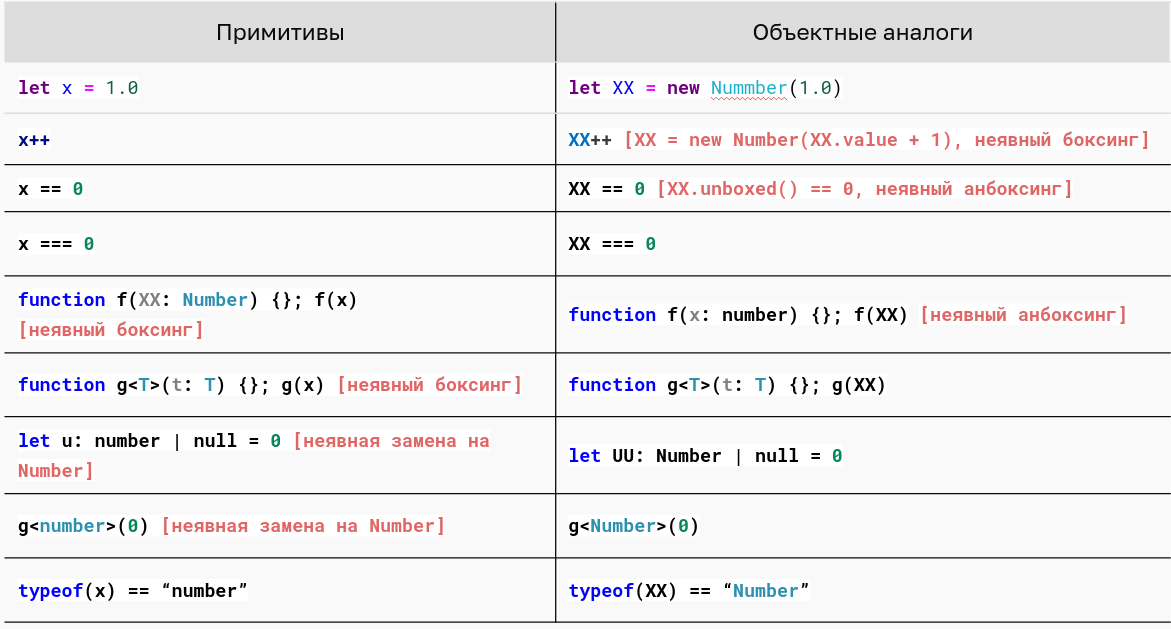
\includegraphics[scale=0.4]{same.png}
    \caption{Выделены места, где ранее выполнялись неявные преобразования}
    \label{fig:example}
\end{figure}

\subsubsection{Новые допустимые конструкции}

\begin{lstlisting}
xx.toStrint() // ошибка компиляции до изменений, будет работать после
xx instanceof Object // ошибка компиляции до изменений, будет работать после
\end{lstlisting}


\subsection{План реализации}
\begin{enumerate}
    \item \textbf{Модификация системы типов}: Убрать примитивные типы на этапе проверки корректности типов в арифметических операциях и преобразованиях типов
    \item \textbf{Обработка констант}: Изменить представление литералов на этапе свёртки констант на объектные типы
    \item \textbf{Оптимизация перед кодогенерацией}: Имплементировать модуль-оптимизацию, где объектные типы будут по возможности заменяться примитивными
\end{enumerate}

\newpage %% Исследование и построение решения задачи
    \section{Описание практической части}
\label{sec:Chapter4} \index{Chapter4}

Компилятор рассматриваемого языка в основном написан на языке программирования C++.

Для наглядности далее в тексте в качестве базового примера будут использоваться типы:
int (примитивный) → Int (объектный аналог)

\subsection{Арифметические операции}
На данном этапе работы было необходимо модифицировать проверку корректности типов в арифметческих операциях:
\begin{itemize}[label={}]
    \item \code{+} , \code{-} , \code{+=} , \code{-=}
    \item \code{++} , \code{--}
    \item \code{*} , \code{/} , \code{\%} , \code{*=}, \code{/=}, \code{\%=}
    \item \code{$\langle \langle$} , \code{$\rangle \rangle$} , \code{$\langle \langle$=} , \code{$\rangle \rangle$=}, \code{$\rangle \rangle \rangle$}, \code{$\rangle \rangle \rangle$=}
    \item \code{|} , \code{|=} , \code{\&} , \code{\&=}, \code{\^}, \code{\^}\code{=}, \code{||} , \code{\&\&}
    \item \code{<} , \code{<=} , \code{>}, \code{>=}, \code{==}, \code{===}, \code{!}
\end{itemize}

В существующей реализации почти в каждой функции проверки производилось безусловное приведение типов операторов к примитивным, поэтому первым этапом работы было удаление или изменение кода, который приводил бы к замене объектных типов на их примитивные аналоги. Далее, основная функция, которая была нужна почти для всех вышеперечисленных операций(исключая логические и унарные) - функция, вычисляющая тип результата бинарного выражения. Ее поведение основывается на иерархии численных типов, оговоренной в спецификации.
Следующий этап заключался в очистке кода от попыток свернуть константы в функциях проверки, чтобы вынести все константные вычисления в отдельный модуль.

\subsection{Преобразования типов}
Для реализации проверки легальности преобразования объектных примитивоподобных типов можно было переиспользовать алгоритм, использовавшийся для проверки преобразований примитивных типов, добавив дополнительные проверки на отношения объектов (Union и Enum).
Структура функции для проверки корректности преобразования представлена на \ref{fig:cmp}
\subsubsection{Основные функции}
\textbf{Вычисление ранга типа}
\begin{lstlisting}[language=C++,caption=GetTypeRank]
/**
 * Проверяет допустимость преобразования между упакованными примитивными типами.
 * Основная идея: проверяет, можно ли безопасно преобразовать один упакованный тип
 * в другой, переисспользуя алгоритмы проверки преобразований для примитивных типов.
 */
bool IsLegalBoxedPrimitiveConversion(Type *target, Type *source) {
    Checker *checker = this->GetChecker()->AsChecker();

    // Проверка на null
    if (target == nullptr || source == nullptr) {
        return false;
    }

    // Обработка union-типов (особый случай)
    if (target->IsUnionType() && source->IsObjectType()) {
        // Получаем базовый примитивный тип для исходного типа
        Type *sourceUnboxed = checker->MaybeUnboxType(source);
        if (!sourceUnboxed || !sourceUnboxed->IsPrimitiveType()) {
            return false;
        }

        // Ищем упакованный тип в union, который можно распаковать
        Type *boxedUnionTarget = target->AsUnionType()->FindUnboxableType();
        if (!boxedUnionTarget) {
            return false;
        }

        // Проверяем совместимость базовых примитивных типов
        Type *targetUnboxed = checker->MaybeUnboxType(boxedUnionTarget);
        return targetUnboxed && targetUnboxed->IsPrimitiveType() &&
               this->IsAssignableTo(sourceUnboxed, target);
    }

    // Оба типа должны быть объектными
    if (!target->IsObjectType() || !source->IsObjectType()) {
        return false;
    }

    // Хотя бы один тип должен быть упакованным примитивом
    if (!target->AsObjectType()->IsBoxedPrimitive() &&
        !source->AsObjectType()->IsBoxedPrimitive()) {
        return false;
    }

    // Получаем базовые примитивные типы
    Type *targetUnboxed = checker->MaybeUnboxType(target);
    Type *sourceUnboxed = checker->MaybeUnboxType(source);

    // Особый случай для int-перечислений
    if (source->IsIntEnumType()) {
        targetUnboxed = checker->GlobalIntType();
    }

    // Проверяем что оба имеют примитивные базовые типы
    if (!targetUnboxed || !sourceUnboxed ||
        !targetUnboxed->IsPrimitiveType() ||
        !sourceUnboxed->IsPrimitiveType()) {
        return false;
    }

    // Проверяем совместимость примитивных типов
    return this->IsAssignableTo(sourceUnboxed, targetUnboxed);
}
\end{lstlisting}
\subsection{Свёртка констант}
Один из основных этапов работы - это имплементация модуля компиляции для сверки констант в начало стадии семантического анализа.
Свёртка констант - вычисление константных выражений с последующей заменой выражений на результаты,
выполняемое на отдельной стадии компиляции. Это оптимизация, которая:
\begin{itemize}[label={--}]
    \item Ускоряет выполнение программы (избегает вычислений в runtime)
    \item Уменьшает размер генерируемого кода
    \item Позволяет обнаружить ошибки на этапе компиляции
\end{itemize}

Исплементированный модуль позволяет рекурсивно обойти const и readonly декларации и заменить константные выражения результатом их вычисления. Алгоритм свёртки констант реализован по аналогии с классическими методами \cite{aho2007}
\subsubsection{Основной алгоритм}
\begin{enumerate}[label={--}]
    \item \textbf{Обход AST} - рекурсивных обход синтаксического дерева программы
    \item \textbf{Идентификация константных выражений} - проверка, можно ли вычислить выражение на этапе компиляции (является ли выражение константным)
    \item \textbf{Вычисление констант} - выполнение операций над константами
    \item \textbf{Замена выражений} - подстановка вычисленных значений вместо исходных выражений
\end{enumerate}

\subsubsection{Поддерживаемые типы и операции}
\textbf{Типы данных}
\begin{itemize}[label={--}]
    \item Числовые литералы (int, float, double)
    \item Символьные литералы (char)
    \item Булевы значения (true/false)
    \item Строковые литералы
    \item Enum значения
\end{itemize}

\textbf{Операции}
\begin{itemize}[label={--}]
    \item Арифметические  +, -, *, /, \%
    \item Битовые  \&, |, \^{}, \~{}, \verb|<<|, \verb|>>|, \verb|>>>|
    \item Логические  \&\&, ||, !
    \item Сравнения  ==, !=, <, >, <=, >=
    \item Унарные  +, -, \~{}
\end{itemize}

\subsubsection{Детали реализации}
\subsubsection*{Типизация и преобразование типов}
\begin{itemize}[label={--}]
    \item Используется система рангов типов TypeRank для определения приоритета преобразований
    \item Реализованы безопасные преобразования между типами с проверкой диапазонов (\cite{krasovsky2022} - Безопасные преобразования типов при свёртке констант требуют проверки диапазонов)
    \item Обработка деления на ноль
\end{itemize}

\begin{lstlisting}[language=C++,caption=Перечисление рангов типов]
enum class TypeRank {
    INT8,
    INT16,
    INT32,
    INT64,
    FLOAT,
    DOUBLE,
    CHAR
};
\end{lstlisting}

\subsubsection{Основные функции}
\textbf{Вычисление ранга типа}
\begin{lstlisting}[language=C++,caption=GetTypeRank]
static TypeRank GetTypeRank(const ir::Literal* lit) {
    if (lit->IsCharLiteral()) {
        return TypeRank::CHAR;
    }

    auto num = lit->AsNumberLiteral()->Number();
    if (num.IsByte()) return TypeRank::INT8;
    if (num.IsShort()) return TypeRank::INT16;
    if (num.IsInt()) return TypeRank::INT32;
    if (num.IsLong()) return TypeRank::INT64;
    if (num.IsFloat()) return TypeRank::FLOAT;
    if (num.IsDouble()) return TypeRank::DOUBLE;
}
\end{lstlisting}

\textbf{Получение значения литерала}
\begin{lstlisting}[language=C++,caption=GetVal]
template <typename TargetType>
static TargetType GetVal(const ir::Literal* node) {
    // Обработка булевых литералов
    if constexpr (std::is_same_v<TargetType, bool>) {
        return node->AsBooleanLiteral()->Value();
    }

    // Обработка символьных литералов
    if constexpr (std::is_same_v<TargetType, char16_t>) {
        return node->AsCharLiteral()->Char();
    }

    auto numNode = node->AsNumberLiteral();

    // Обработка числовых литералов разных типов
    if constexpr (std::is_same_v<TargetType, int8_t>) {
        return numNode->Number().GetByte();
    }
    if constexpr (std::is_same_v<TargetType, int16_t>) {
        return numNode->Number().GetShort();
    }
    // ...
    if constexpr (std::is_same_v<TargetType, double>) {
        return numNode->Number().GetDouble();
    }
}
\end{lstlisting}

\textbf{Преобразование значений между типами}
\begin{lstlisting}[language=C++,caption=CastValTo]
template <typename To>
static To CastValTo(const ir::Literal* lit) {
    // Обработка булевых литералов
    if (lit->IsBooleanLiteral()) {
        return static_cast<To>(GetVal<bool>(lit));
    }

    // Определение ранга типа и преобразование
    auto rank = GetTypeRank(lit);
    switch (rank) {
        case TypeRank::DOUBLE:
            return static_cast<To>(GetVal<double>(lit));
        case TypeRank::FLOAT:
            return static_cast<To>(GetVal<float>(lit));
        // ...
        case TypeRank::CHAR:
            return static_cast<To>(GetVal<char16_t>(lit));
    }
}
\end{lstlisting}


\subsubsection*{Обработка ошибок}
\begin{itemize}[label={--}]
    \item Генерация диагностических сообщений для недопустимых операций
    \item Реализованы безопасные преобразования между типами с проверкой диапазонов
    \item Отдельные функции преобразований между целыми и вещественными типами
\end{itemize}

\subsubsection*{Оптимизации}
\begin{itemize}[label={--}]
    \item Использование битовых операций для безопасной работы с целыми числами
    \item Специальная обработка строковых конкатенаций
    \item Оптимизация шаблонных литералов
\end{itemize}

\subsection{Оптимизация}


Реализованная оптимизация представляет собой систему преобразования типов, которая рекурсивно анализирует и модифицирует абстрактное синтаксическое дерево (AST) для выполнения операций nboxing (распаковки) и boxing (упаковки) типов.

\subsection*{Архитектура оптимизации}

\subsubsection{Класс UnboxVisitor}
Рекурсивный анализ дерева проводится с помощью специального класса \texttt{UnboxVisitor}, реализующего методы \texttt{VisitX} для различных типов узлов AST. Его задачи:
\begin{enumerate}
    \item Обойти AST и найти места, где можно заменить boxed-типы на примитивы
    \item Вставить явные преобразования (например, вызовы \texttt{unboxed()}, \texttt{valueOf()}, intrinsic-функции)
    \item Обновить соответствующие типы в выражениях, объявлениях и сигнатурах
    \item Заново запустить функцию валидации ноды
\end{enumerate}

Подобный подход к преобразованию типов используется в TypeScript \cite{typescript_doc}
\subsubsection{Обрабатываемые узлы AST}
Примеры обрабатываемых узлов:
\begin{itemize}
    \item \texttt{VisitCallExpression} — вызовы функций
    \item \texttt{VisitBinaryExpression} — бинарные операции (+, ==, \&\& и т. д.)
    \item \texttt{VisitMemberExpression} — доступ к полям/методам (\texttt{obj.field}, \texttt{arr[index]})
    \item \texttt{VisitReturnStatement} — возвращаемые значения
    \item \texttt{VisitVariableDeclarator} — объявления переменных
\end{itemize}

\subsubsection{Механизм работы Visitor'ов}

Каждый узел AST имеет метод \texttt{Accept(visitor)}.
При вызове \texttt{astNode->Accept(visitor)} управление передаётся в соответствующий метод \texttt{VisitX} у UnboxVisitor.

\subsubsection{Пример обработки CallExpression}
\begin{lstlisting}[language=C++,caption=Обработка вызовов функций]
void VisitCallExpression(ir::CallExpression *call) override {
    // 1. Обновление типов аргументов
    for (size_t i = 0; i < call->Arguments().size(); i++) {
        auto *arg = call->Arguments()[i];
        auto *expectedType = call->Signature()->Params()[i]->TsType();
        call->Arguments()[i] = AdjustType(uctx_, arg, expectedType);
    }

    // 2. Обновление возвращаемого типа
    if (call->Signature()->ReturnType()->IsPrimitiveType()) {
        call->SetTsType(call->Signature()->ReturnType());
    }
}
\end{lstlisting}

\subsubsection{Логика преобразования типов}
Решение о том, нужно ли вставлять boxing, unboxing или конверсию примитивов, принимается с помощью метода AdjustType:
\begin{lstlisting}[language=C++,caption=Метод AdjustType]
static ir::Expression *AdjustType(UnboxContext *uctx,
                                ir::Expression *expr,
                                checker::Type *expectedType) {
    // Если выражение — примитив, а ожидается объект → boxing
    if (expr->TsType()->IsPrimitiveType()
        && expectedType->IsObjectType()) {
        return InsertBoxing(uctx, expr);
    }
    // Если выражение — boxed-объект, а нужен примитив → unboxing
    if (TypeIsBoxedPrimitive(expr->TsType())
        && expectedType->IsPrimitiveType()) {
        return InsertUnboxing(uctx, expr);
    }
    // Если оба примитива, но разных типов → конверсия
    if (expr->TsType()->IsPrimitiveType()
        && expectedType->IsPrimitiveType()) {
        return InsertPrimitiveConversion(uctx, expr, expectedType);
    }
    return expr;
}
\end{lstlisting}

\subsubsection{Пример преобразования}

\textbf{Исходный код}
\begin{lstlisting}[language=TypeScript]
let x: Int = 10;  // Int — объектный тип
let y: int = x + 5;   // int — примитив
\end{lstlisting}

\textbf{Преобразование AST}
\begin{lstlisting}[caption=AST до оптимизации]
BinaryExpression(
    left: Identifier("x", type=Int),
    op: +,
    right: NumberLiteral(5, type=int)
)
\end{lstlisting}


\begin{lstlisting}[caption=AST после оптимизации]
    BinaryExpression(
        left: CallExpression(
            callee: MemberExpression(
                object: Identifier("x", type=Int),
                property: "unboxed"
            ),
            type=int
        ),
        op: +,
        right: NumberLiteral(5, type=int)
    )
\end{lstlisting}

\subsection{Тестирование}
Все необходимые тестовые сценарии, покрывающие работу языка с примитивными и объектными типами, были сделаны на основе уже существующих тестов с небольшими правками синтаксиса. Устаревшие тесты были удалены или переработаны в соответствие с новой семантикой.

\subsection{Замеры производительности}
Результаты запусков бенчмарков с помощью уже существующих внутриплатформенных инструментов тестирования показали прирост показателей времени компиляции:
\begin{itemize}[label={--}]
    \item \textbf{Just In Time компиляция (JIT)}: ускорение на 8.000\%
    \item \textbf{Ahead Of Time компиляция (AOT)}: ускорение на 10.2\%
    \item \textbf{Just In Time компиляция (JIT)}: ускорение на 14.6\%
\end{itemize}

\newpage %% Описание практической части
    \section{Заключение}
\label{sec:Chapter5} \index{Chapter5}

бебебебебе ляляляляля

\newpage
 %% Заключение

    %% НЕ ТРОГАЙТЕ!!!
    \nocite{*}
    \printbibliography
    %% в зависимости от надобности подключаем раздел "Приложение"
    % \newpage
    % \section*{Приложение}
\addcontentsline{toc}{section}{Приложение}
\label{sec:Apendix} \index{Apendix}
абабабаба
\end{document}
